% audio_pipeline.tex — Phase-3 inference: inputs, processing, output.
\documentclass[tikz,border=8pt]{standalone}
\usepackage{amsmath}
\usetikzlibrary{positioning,arrows.meta}
\definecolor{ink}{HTML}{1A1A1A}
\definecolor{muted}{HTML}{6B7280}
\definecolor{okblue}{HTML}{0072B2}
\definecolor{okamber}{HTML}{E69F00}
\definecolor{okverm}{HTML}{D55E00}
\definecolor{okgreen}{HTML}{009E73}
\begin{document}
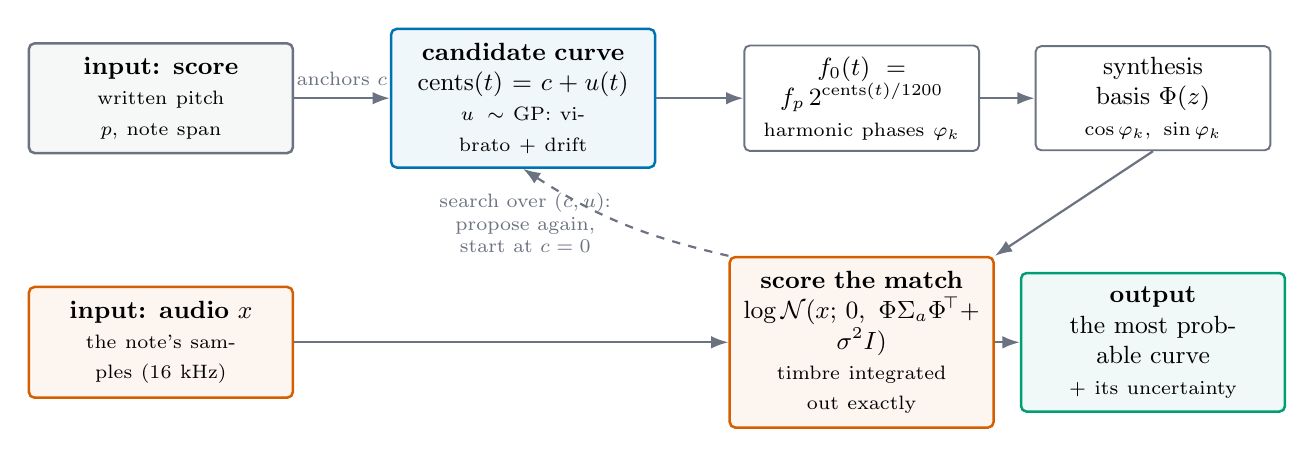
\begin{tikzpicture}[font=\small,
  box/.style={draw=#1, line width=0.9pt, rounded corners=2pt, fill=#1!6,
              align=center, inner sep=5pt, text width=30mm},
  op/.style={draw=muted, line width=0.7pt, rounded corners=2pt,
             align=center, inner sep=4pt, text width=27mm, fill=white},
  arr/.style={-{Latex[length=2.2mm,width=1.6mm]}, draw=muted, line width=0.8pt},
]
\node[box=muted] (score) at (0, 1.6)
  {\textbf{input: score}\\ \scriptsize written pitch $p$, note span};
\node[box=okblue] (cand) at (4.6, 1.6)
  {\textbf{candidate curve}\\ $\mathrm{cents}(t) = c + u(t)$\\
   \scriptsize $u \sim$ GP: vibrato + drift};
\node[op] (f0) at (8.9, 1.6)
  {$f_0(t) = f_p \, 2^{\mathrm{cents}(t)/1200}$\\
   \scriptsize harmonic phases $\varphi_k$};
\node[op] (phi) at (12.6, 1.6)
  {synthesis basis $\Phi(z)$\\ \scriptsize $\cos\varphi_k,\ \sin\varphi_k$};
\node[box=okverm] (audio) at (0, -1.5)
  {\textbf{input: audio} $x$\\ \scriptsize the note's samples (16 kHz)};
\node[box=okverm] (lik) at (8.9, -1.5)
  {\textbf{score the match}\\
   $\log \mathcal N(x;\, 0,\ \Phi \Sigma_a \Phi^{\!\top} \!+ \sigma^2 I)$\\
   \scriptsize timbre integrated out exactly};
\node[box=okgreen] (out) at (12.6, -1.5)
  {\textbf{output}\\ the most probable curve\\ \scriptsize + its uncertainty};
\draw[arr] (score) -- node[above, font=\scriptsize, text=muted, yshift=1pt]
  {anchors $c$} (cand);
\draw[arr] (cand) -- (f0);
\draw[arr] (f0) -- (phi);
\draw[arr] (phi.south) -- (lik.north east);
\draw[arr] (audio) -- (lik);
\draw[arr] (lik) -- (out);
\draw[arr, dashed] (lik.north west) to[bend left=10]
  node[left, font=\scriptsize, text=muted, align=center]
  {search over $(c, u)$:\\ propose again,\\ start at $c = 0$} (cand.south);
\end{tikzpicture}
\end{document}
